\documentclass[../review_3.tex]{subfiles}
\graphicspath{{\subfix{../img/}}}
\begin{document}

\chapter{Einleitung}\thispagestyle{fancy}

\section{Problemstellung}
Denial-of-Service-Angriffe stellen eine ernstzunehmende und stetig wachsende Bedrohung dar.
Im digitalen Zeitalter sind viele Systeme über das Internet oder private Netzwerke miteinander verbunden. Viele Unternehmen, Krankenhäuser und Behörden sind durch unzureichende Schutzmaßnahmen und große Wirkung zu beliebten Angriffszielen geworden\cite{infopoint_security_cyber_angriffe}. Bei solchen Angriffen werden in der Regel finanzielle oder auch politische Gründe verfolgt, selten aber auch die bloße Störung oder Destruktion des Ziels.

Bei DoS\footnote{Denial of Service, dt.: Verweigerung des Dienstes, Nichtverfügbarkeit des Dienstes}- und DDoS\footnote{Distributed Denial of Service}-Attacken werden Server und Infrastrukturen mit einer Flut sinnloser Anfragen so stark überlastet, dass sie von ihrem normalen Betrieb abgebracht werden. Daraus kann resultieren, dass Nutzer die angebotenen Dienste des Betreibers nicht mehr erreichen und Daten bei dem Angriff verloren gehen können.
Hierbei können schon schwache Rechner große Schaden bei deutlich leistungsfähigeren Empfängern auslösen. In Botnetzen können die Angriffe zusätzlich von mehreren Computern gleichzeitig koordiniert werden, aus verschiedensten Netzwerken stammen \cite{tecchannel_gefahr_botnet} und damit gleichzeitig die Angriffskraft verstärken und die Erkennung erschweren.

Das Ungleichgewicht zwischen der Einfachheit bei der Erzeugung von Angriffen gegenüber komplexer und ressourcenintensiver DoS-Abwehr verschärft das Problem zusätzlich. Obwohl gelegentlich Erfolge im Kampf gegen DoS-Angriffe erzielt werden (z.B. Stilllegung einiger großer \glqq DoS-for-Hire\grqq{} Webseiten), vergrößert sich das Datenvolumen der DoS-Angriffe stetig weiter. Allein zwischen 2014 und 2017 hat sich die Frequenz von DoS-Angriffen um den Faktor 2,5 vergrößert und das Angriffsvolumen verdoppelt sich fast jährlich \cite{neustar_ddos_report}. Die Schäden werden weltweit zwischen 20.000 und 40.000 US-Dollar pro Stunde geschätzt \cite{datacenterknowledge_study}.

Im Bereich kommerzieller DoS-Abwehr haben sich einige Ansätze hervorgetan (z.B. Project Shield\cite{projectshield}, Cloudflare\cite{cloudflare} oder AWS Shield\cite{aws_shield}). Der Einsatz kommerzieller Lösungen birgt jedoch einige Probleme, etwa mitunter erhebliche Kosten oder das Problem des notwendigen Vertrauens, welches dem Betreiber einer DoS-Abwehr entgegengebracht werden muss. Folglich ist eine effiziente Abwehr von DoS-Angriffen mit eigenen Mitteln ein oft gewünschtes Ziel - insbesondere wenn sich dadurch mehrere Systeme zugleich schützen lassen.

Ziel dieses Softwareprojekts ist es, ein System zwischen der Internet-Anbindung und dem internem Netzwerk zu schaffen, das bei einer hohen Bandbreite und im Dauerbetrieb effektiv (D)DoS Angriffe abwehren kann, während Nutzer weiterhin ohne Einschränkungen auf ihre Dienste zugreifen können. Die entstehende Anwendung implementiert eine (D)DoS-Verkehrs-Inspektion und einen intelligenten Regelgenerator, wodurch interne Netzwerke vor externen Bedrohungen, die zu einer Überlastung des Systems führen würden, geschützt sind. Es enthält Algorithmen zur Verkehrsanalyse, die bösartigen Verkehr erkennen und ausfiltern können, ohne die Benutzererfahrung zu beeinträchtigen und ohne zu Ausfallzeiten zu führen.

\section{Überblick}

\begin{figure}[H]
    \centering
    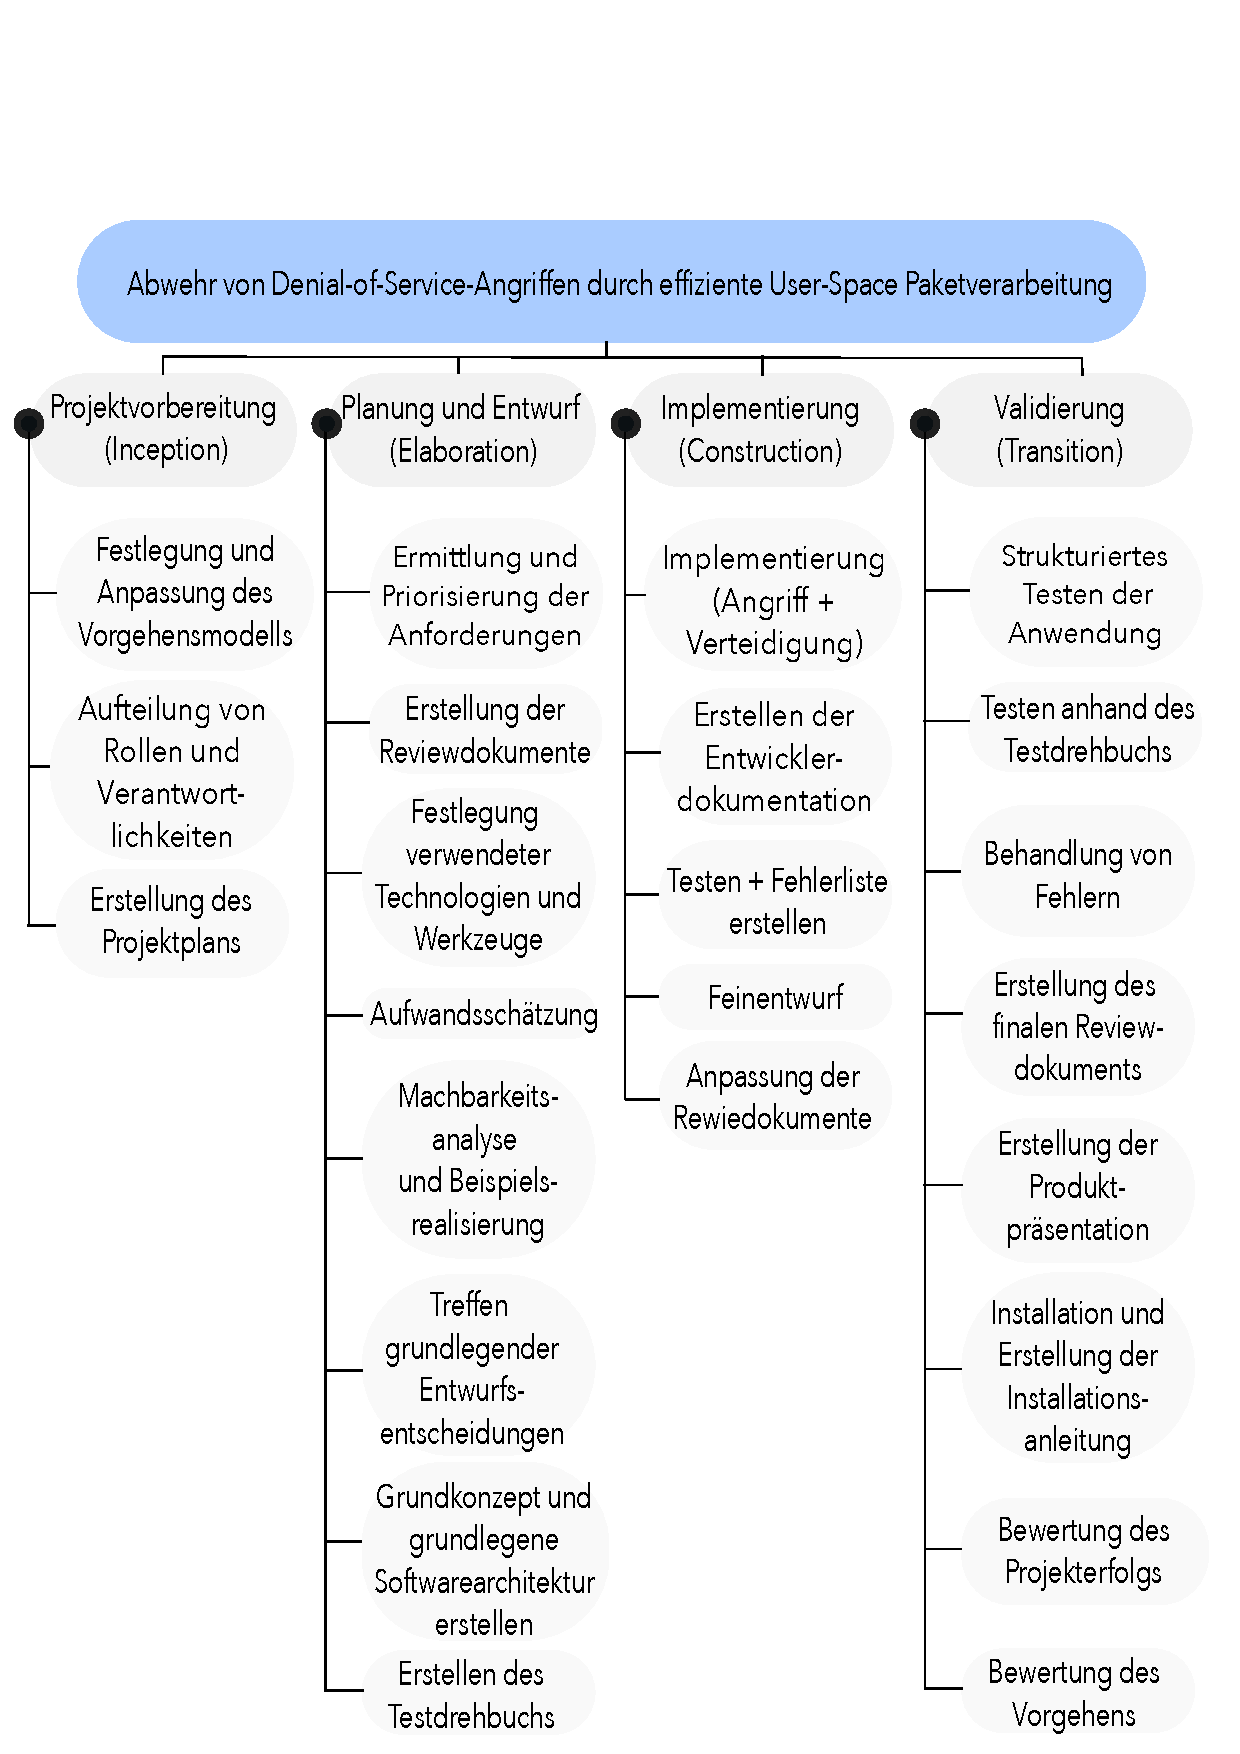
\includegraphics[width=0.8\linewidth]{img/projektstrukturplan.pdf}
    \caption{Projektstrukturplan}
    \label{projektstrukturplan}
\end{figure}

Das Softwareprojekt wurde vom zuständigen Fachgebiet in drei Teile aufgeteilt. Die Planungs- und Entwicklungsphase, die Implementierungsphase und die Validierungsphase dauern jeweils einen Monat und werden durch ein Review abgeschlossen. Zu diesen Reviews werden die Ergebnisse der vergangenen Phase vorgestellt und die erforderlichen Review-Dokumente abgegeben.

Zu Beginn des Projekts wurde sich auf den Unified Process als Vorgehensmodell geeinigt, damit sowohl ein gewisser Grad an Flexibilität als auch die Planbarkeit der Ergebnisse gewährleistet werden kann. Prinzipiell besteht dieses Vorgehensmodell aus vier Phasen, von denen die Konzeption und die Ausarbeitung beide in der Planungs- und Entwurfsphase lagen. Die Konstruktionsphase und die Inbetriebnahme decken sich zeitlich mit der Implementierungs- und der Validierungsphase.

Dieses dritte Review-Dokument bezieht sich auf die Validierungssphase. Das heißt, dass es auf den Ergebnissen der vorhergehenden Phase und dem zweiten Review-Dokument vom 23. Juni 2021 aufbaut.

Das erste Review-Dokument enthält die gängigen Inhalte eines Pflichtenhefts wie die funktionalen und nicht-funktionalen Anforderungen, eine Aufwands- und Risikoanalyse und Überlegungen zum Vorgehen und der internen Organisation. Außerdem umfasst es eine Entwurfsdokumentation für den Grobentwurf, die Anforderungsanalyse, ein Kapitel zu den Technologien und Entwicklungswerkzeugen, Ergebnisse zu den Machbarkeitsanalysen und Beispielrealisierungen und ein Testdrehbuch.

Im zweiten Review-Dokument werden im Kapitel zum Grobentwurf zusätzlich zur erneuten Erläuterung der grundlegenden Architektur die für den Unified Process üblichen Überarbeitungen des Grobentwurfs dargestellt und begründet. Dabei wird, genauso wie beim darauffolgenden Feinentwurf, Paket für Paket vorgegangen. Schließlich werdeb in einem Bug-Review die offenen Anforderungen und Fehler beschrieben und die mittels des Tools Kimai erfassten Arbeitszeiten ausgewertet.

In diesem dritten Review-Dokument kommt nun ein ausführliches Kapitel zu sämtlichen Tests dazu. Außerdem behandelt es verschiedene Softwaremetriken und Statistiken, wie Konventionen und den Umfang der Software. Das Kapitel zur Auswertung der erfassten Arbeitszeiten enthält nun auch diese letzte Phase des Softwareprojekts. Am Ende des Dokuments kommt es zu einer umfangreichen Auswertung des Projekts.

Es bleibt also anzumerken, dass einige Teile dieses Dokuments dem ersten und zweiten Review-Dokument entnommen sind, weil dies vom Fachgebiet empfohlen wurde und dadurch die Veränderungen besonders gut dargestellt werden können.

Die Erstellung dieses Review-Dokuments stellt allerdings nur einen Teil der in dieser Phase erledigten Aufgaben dar. Hauptsächlich ging es um das Testen, aber auch um weitere Themen, was sich im Projektstrukturplan in Abb. \ref{projektstrukturplan} gut erkennen lässt.

\end{document}
